%%% The main file. It contains definitions of basic parameters and includes all other parts.

%% Settings for single-side (simplex) printing
% Margins: left 40mm, right 25mm, top and bottom 25mm
% (but beware, LaTeX adds 1in implicitly)
\documentclass[12pt,a4paper]{report}
\setlength\textwidth{145mm}
\setlength\textheight{247mm}
\setlength\oddsidemargin{15mm}
\setlength\evensidemargin{15mm}
\setlength\topmargin{0mm}
\setlength\headsep{0mm}
\setlength\headheight{0mm}
% \openright makes the following text appear on a right-hand page
\let\openright=\clearpage

%% Settings for two-sided (duplex) printing
% \documentclass[12pt,a4paper,twoside,openright]{report}
% \setlength\textwidth{145mm}
% \setlength\textheight{247mm}
% \setlength\oddsidemargin{14.2mm}
% \setlength\evensidemargin{0mm}
% \setlength\topmargin{0mm}
% \setlength\headsep{0mm}
% \setlength\headheight{0mm}
% \let\openright=\cleardoublepage

%% Generate PDF/A-2u
\usepackage[a-2u]{pdfx}

%% Character encoding: usually latin2, cp1250 or utf8:
\usepackage[utf8]{inputenc}

%% Prefer Latin Modern fonts
\usepackage{lmodern}

%% Further useful packages (included in most LaTeX distributions)
\usepackage{amsmath}        % extensions for typesetting of math
\usepackage{amsfonts}       % math fonts
\usepackage{amsthm}         % theorems, definitions, etc.
\usepackage{bbding}         % various symbols (squares, asterisks, scissors, ...)
\usepackage{bm}             % boldface symbols (\bm)
\usepackage{graphicx}       % embedding of pictures
\usepackage{fancyvrb}       % improved verbatim environment
\usepackage{natbib}         % citation style AUTHOR (YEAR), or AUTHOR [NUMBER]
\usepackage[nottoc]{tocbibind} % makes sure that bibliography and the lists
			    % of figures/tables are included in the table
			    % of contents
\usepackage{dcolumn}        % improved alignment of table columns
\usepackage{booktabs}       % improved horizontal lines in tables
\usepackage{paralist}       % improved enumerate and itemize
\usepackage{xcolor}         % typesetting in color

%\usepackage{csquotes}
%todo notes
\usepackage[colorinlistoftodos,prependcaption,textsize=tiny]{todonotes}
%\newcommand{\todo}[2][1=]{\todo[linecolor=red,backgroundcolor=red!25,bordercolor=red,#1]{#2}}
%\newcommand{\unsure}[2][1=]{\todo[linecolor=blue,backgroundcolor=blue!25,bordercolor=blue,#1]{#2}}
%\newcommandx{\idea}[2][1=]{\todo[linecolor=OliveGreen,backgroundcolor=OliveGreen!25,bordercolor=OliveGreen,#1]{#2}}
\usepackage{makecell}
\usepackage{array}
\newcolumntype{P}[1]{>{\centering\arraybackslash}p{#1}}

\newcommand{\relationcell}[3]{\textbf{#1} \newline  #2 \newline \textit{{\footnotesize #3}}}
\newcommand{\relationcelltacred}[2]{\textbf{#1} \newline \textit{ {\footnotesize #2}}}
\newcommand{\freqencycell}[2]{#1\% \newline (#2)}
\usepackage{longtable}


%%% Basic information on the thesis

% Thesis title in English (exactly as in the formal assignment)
\def\ThesisTitle{Entity Relationship Extraction}

% Author of the thesis
\def\ThesisAuthor{Zuzana Šimečková}

% Year when the thesis is submitted
\def\YearSubmitted{2020}

% Name of the department or institute, where the work was officially assigned
% (according to the Organizational Structure of MFF UK in English,
% or a full name of a department outside MFF)
\def\Department{Institute of Formal and Applied Linguistics}

% Is it a department (katedra), or an institute (ústav)?
\def\DeptType{Institute}

% Thesis supervisor: name, surname and titles
\def\Supervisor{RNDr. Milan Straka, Ph.D.}

% Supervisor's department (again according to Organizational structure of MFF)
\def\SupervisorsDepartment{Institute of Formal and Applied Linguistics}

% Study programme and specialization
\def\StudyProgramme{Computer Science}
\def\StudyBranch{IUI}

% An optional dedication: you can thank whomever you wish (your supervisor,
% consultant, a person who lent the software, etc.)
\def\Dedication{%
Dedication.
}

% Abstract (recommended length around 80-200 words; this is not a copy of your thesis assignment!)
\def\Abstract{%
Abstract.
}

% 3 to 5 keywords (recommended), each enclosed in curly braces
\def\Keywords{%
{key} {words}
}

%% The hyperref package for clickable links in PDF and also for storing
%% metadata to PDF (including the table of contents).
%% Most settings are pre-set by the pdfx package.
\hypersetup{unicode}
\hypersetup{breaklinks=true}

% Definitions of macros (see description inside)
%%% This file contains definitions of various useful macros and environments %%%
%%% Please add more macros here instead of cluttering other files with them. %%%

%%% Minor tweaks of style

% These macros employ a little dirty trick to convince LaTeX to typeset
% chapter headings sanely, without lots of empty space above them.
% Feel free to ignore.
\makeatletter
\def\@makechapterhead#1{
  {\parindent \z@ \raggedright \normalfont
   \Huge\bfseries \thechapter. #1
   \par\nobreak
   \vskip 20\p@
}}
\def\@makeschapterhead#1{
  {\parindent \z@ \raggedright \normalfont
   \Huge\bfseries #1
   \par\nobreak
   \vskip 20\p@
}}
\makeatother

% This macro defines a chapter, which is not numbered, but is included
% in the table of contents.
\def\chapwithtoc#1{
\chapter*{#1}
\addcontentsline{toc}{chapter}{#1}
}

% Draw black "slugs" whenever a line overflows, so that we can spot it easily.
\overfullrule=1mm

%%% Macros for definitions, theorems, claims, examples, ... (requires amsthm package)

\theoremstyle{plain}
\newtheorem{thm}{Theorem}
\newtheorem{lemma}[thm]{Lemma}
\newtheorem{claim}[thm]{Claim}

\theoremstyle{plain}
\newtheorem{defn}{Definition}

\theoremstyle{remark}
\newtheorem*{cor}{Corollary}
\newtheorem*{rem}{Remark}
\newtheorem*{example}{Example}

%%% An environment for proofs

\newenvironment{myproof}{
  \par\medskip\noindent
  \textit{Proof}.
}{
\newline
\rightline{$\qedsymbol$}
}

%%% An environment for typesetting of program code and input/output
%%% of programs. (Requires the fancyvrb package -- fancy verbatim.)

\DefineVerbatimEnvironment{code}{Verbatim}{fontsize=\small, frame=single}

%%% The field of all real and natural numbers
\newcommand{\R}{\mathbb{R}}
\newcommand{\N}{\mathbb{N}}

%%% Useful operators for statistics and probability
\DeclareMathOperator{\pr}{\textsf{P}}
\DeclareMathOperator{\E}{\textsf{E}\,}
\DeclareMathOperator{\var}{\textrm{var}}
\DeclareMathOperator{\sd}{\textrm{sd}}

%%% Transposition of a vector/matrix
\newcommand{\T}[1]{#1^\top}

%%% Various math goodies
\newcommand{\goto}{\rightarrow}
\newcommand{\gotop}{\stackrel{P}{\longrightarrow}}
\newcommand{\maon}[1]{o(n^{#1})}
\newcommand{\abs}[1]{\left|{#1}\right|}
\newcommand{\dint}{\int_0^\tau\!\!\int_0^\tau}
\newcommand{\isqr}[1]{\frac{1}{\sqrt{#1}}}

%%% Various table goodies
\newcommand{\pulrad}[1]{\raisebox{1.5ex}[0pt]{#1}}
\newcommand{\mc}[1]{\multicolumn{1}{c}{#1}}


% Title page and various mandatory informational pages
\begin{document}
%%% Title page of the thesis and other mandatory pages

%%% Title page of the thesis

\pagestyle{empty}
\hypersetup{pageanchor=false}
\begin{center}

\centerline{\mbox{
\includegraphics[width=166mm]{./img/logo-en.pdf}}}

\vspace{-8mm}
\vfill

{\bf\Large MASTER THESIS}

\vfill

{\LARGE\ThesisAuthor}

\vspace{15mm}

{\LARGE\bfseries\ThesisTitle}

\vfill

\Department

\vfill

{
\centerline{\vbox{\halign{\hbox to 0.45\hsize{\hfil #}&\hskip 0.5em\parbox[t]{0.45\hsize}{\raggedright #}\cr
Supervisor of the master thesis:&\Supervisor \cr
\noalign{\vspace{2mm}}
Study programme:&\StudyProgramme \cr
\noalign{\vspace{2mm}}
Study branch:&\StudyBranch \cr
}}}}

\vfill

% Zde doplňte rok
Prague \YearSubmitted

\end{center}

\newpage

%%% Here should be a bound sheet included -- a signed copy of the "master
%%% thesis assignment". This assignment is NOT a part of the electronic
%%% version of the thesis. DO NOT SCAN.
This is not a~part of the electronic version of the thesis, do not scan!

%%% A page with a solemn declaration to the master thesis

\openright
\hypersetup{pageanchor=true}
\pagestyle{plain}
\pagenumbering{roman}
\vglue 0pt plus 1fill

\noindent
I declare that I carried out this master thesis independently, and only with the cited
sources, literature and other professional sources. It has not been used to obtain another
or the same degree.

\medskip\noindent
I understand that my work relates to the rights and obligations under the Act No.~121/2000 Sb.,
the Copyright Act, as amended, in particular the fact that the Charles
University has the right to conclude a license agreement on the use of this
work as a school work pursuant to Section 60 subsection 1 of the Copyright~Act.

\vspace{10mm}

\hbox{\hbox to 0.5\hsize{%
In \hbox to 6em{\dotfill} date \hbox to 6em{\dotfill}
\hss}\hbox to 0.5\hsize{\dotfill\quad}}
\smallskip
\hbox{\hbox to 0.5\hsize{}\hbox to 0.5\hsize{\hfil Author's signature\hfil}}

\vspace{20mm}
\newpage

%%% Dedication

\openright

\noindent
\Dedication

\newpage

%%% Mandatory information page of the thesis

\openright

\vbox to 0.5\vsize{
\setlength\parindent{0mm}
\setlength\parskip{5mm}

Title:
\ThesisTitle

Author:
\ThesisAuthor

\DeptType:
\Department

Supervisor:
\Supervisor, \SupervisorsDepartment

Abstract:
\Abstract

Keywords:
\Keywords

\vss}

\newpage

\openright
\pagestyle{plain}
\pagenumbering{arabic}
\setcounter{page}{1}


%%% A page with automatically generated table of contents of the master thesis

\tableofcontents

%%% Each chapter is kept in a separate file
\chapter*{Introduction}
\addcontentsline{toc}{chapter}{Introduction}

There has been made noticeable progress in natural language processing since the first deep neural networks attempts. With multiple new approaches and \todo{not a sentence} inventions such as multitask learning, word embeddings, RNN, attention and the transformer architecture.   Last year \cite{devlin2018bert} created BERT and managed to achieve state-of-the-art performance in eleven natural language processing tasks, including GLUE (7.7\% point absolute improvement), MultiNLI accuracy (4.6\% absolute improvement) and SQuAD problems.


In this thesis, we will try to use those novel approaches to predict relation between two entities based on a Czech sentence. First part of this thesis will be focused on data. We will  introduce some existing English datasets for Entity Relation Extraction. Than we will describe how we prepared data for Czech version of this task using distant supervision on Czech Wikipedia and Wikidata. Second part \todo{o čem bude druhá část}


\chapter{Relationship extraction intro} \todo{změnit název}

\section{Terminology}
Terminology in NLP subtasks is often not exact or non-standardized. We will attempt to introduce the following concepts as exactly as possible while respecting the terms that seem to be established by the majority. \todo{hloupá věta}

\todo{někam zapracovat příklad na větě, jak je nejdřív najití rozštíření a tak všechno}

\defineterm{Relation} in this context is semantic (not grammatical etc.). It has a type, is binary and oriented, and describes the relationship between a subject and an object of the relationship. We will use the word relation as an equivalent for its type and the term relationship for an instance of the relation. 

\defineterm{Subject} and \defineterm{Object}. The subject is the first argument of a relation, the object is the second. In the sentence \vuvozovkach{Albus Severus is Harry Potters's son.} a relation of type\relationtype{son} is captured, the subject is John and the object is Eric. The reasoning for this choice of direction is as follows: suppose we are gathering information about Harry, then we would probably have both the information that his son is Albus Severus and that his father is James. So we are gathering information about the subject (Harry Potter), even though in most sentences Harry is likely to be the grammatical object: \vuvozovkach{James is Harry's father.} We will use the notation \relation{relation type}{subject}{object}: \relation{son}{Harry Potter}{Albus Severus Potter}. \todo{will we, lepší vzhled}

Both the subject and the object can generally be any word or sequence of words that represent concepts that have the ability to form relations. In some cases subjects, objects, or both are limited to entities or named entities.

\defineterm{Named entity} \todo{ukradeno z wiki, ocitovat nebo ukráct od jinud}  is a real-world object, such as persons, locations, organizations, products, etc., that can be denoted with a proper name. It can be abstract or have a physical existence. Named entities can simply be viewed as entity instances (e.g., New York City is an instance of a city). Sometimes, numeric data is considered in this category as well (for example by Named Entity Recognition tools). An \defineterm{entity} is a named entity whose proper name is unknown or unimportant but still is an entity instance. \todo{definice kruhem}

\defineterm{Relation inventory} is the set of relations, that are considered valid for a given dataset or model.

\defineterm{Positive relation mention} is a sentence, that captures a relationship: a relation together with a tagged subject and object. We will omit the word positive unless we want to emphasize the fact.

\defineterm{Negative mention} is close to relation mention in the sense that it is a sentence with tagged subject and object, but the relation type is one of these types: \todo{odrážky}
\begin{itemize}
\item \relationtype{other} - human annotator would classify a relation, that is not in inventory.
\item \relationtype{no relation} - in this case, human annotators should feel an absence of a relationship between a subject and an object. \todo{doplnit příklady, včetně vyloženě ne příkladu}



\end{itemize}

\relationtype{No relation} comes with difficulties. Since there is no semantic relationship between subject and object, it makes it harder to choose subject-object pairs. It is probably desirable to have subject-object pairs, that could be related in a different sentence.

\defineterm{Relationship Extraction} \todo{znímit entity z názvu}

\defineterm{Lemma} \todo{A form from a lexeme chosen by convention (e.g.,
nominative singular for nouns, infinitive for verbs) to represent that
set.
Also called the canonical/base/dictionary/citation form. For every
form, there is a corresponding lemma}

\defineterm{Lexeme}\todo{An abstract entity; the set of all forms related by
inflection (but not derivation).
}

\defineterm{Noun phrase}
\section{Czech language}
One of the objectives of this thesis is to work with Czech language, therefore we find it useful to make some notes on Czech (for non-Czech speaking readers). Czech is a Slavic language with rich morphology and relatively free word order. Most of Czech morphology can be treated with a morphological analyzer, still, it might be useful to have a better understanding of the language we will work with.

\subsection{Inflection}
In Czech, nouns, adjectives, pronounce and numerals are declined. The inflection expresses (not necessarily unambiguously) one of seven cases and a number (singular or plural). Any inflected word in Czech has a grammatical gender, for words, that have natural gender, those two genders align: \vuvozovkach{žena} (\textit{woman}) is feminine and \vuvozovkach{muž} (\textit{man}) is masculine. The inflection of each declinable word follows a pattern. This all means that a single word (lemma) can have a lexeme of size \todo{kolik?}

Verbs are conjugated, the conjugation expresses person, numeral, tense, voice, and mode. Verbs follow one of 14 patterns. An average Czech either finds the theory about Czech verbs and tenses confusing or is even unaware of the existence of the verb patterns, some verbs tend to be used in a grammatically incorrect forms even in the official language.

An important aspect of declension for us is agreement. In English, subject and verb agree (limited just to the third person). In Czech, subject and verb also agree, but in noun phrases there needs to be an agreement as well. \todo{příklad: toho, jak je nějaká noun phrase, počet lexémů, počet validních .. } \todo{odkaz dopředu, kde řeším, jak matchovat}

\subsection{Free word order}

\todo{https://www.aclweb.org/anthology/P14-5003.pdf, statistiky o češtině}
\chapter{Title of the second chapter}

\section{Title of the first subchapter of the second chapter}

\begin{figure}[p]\centering
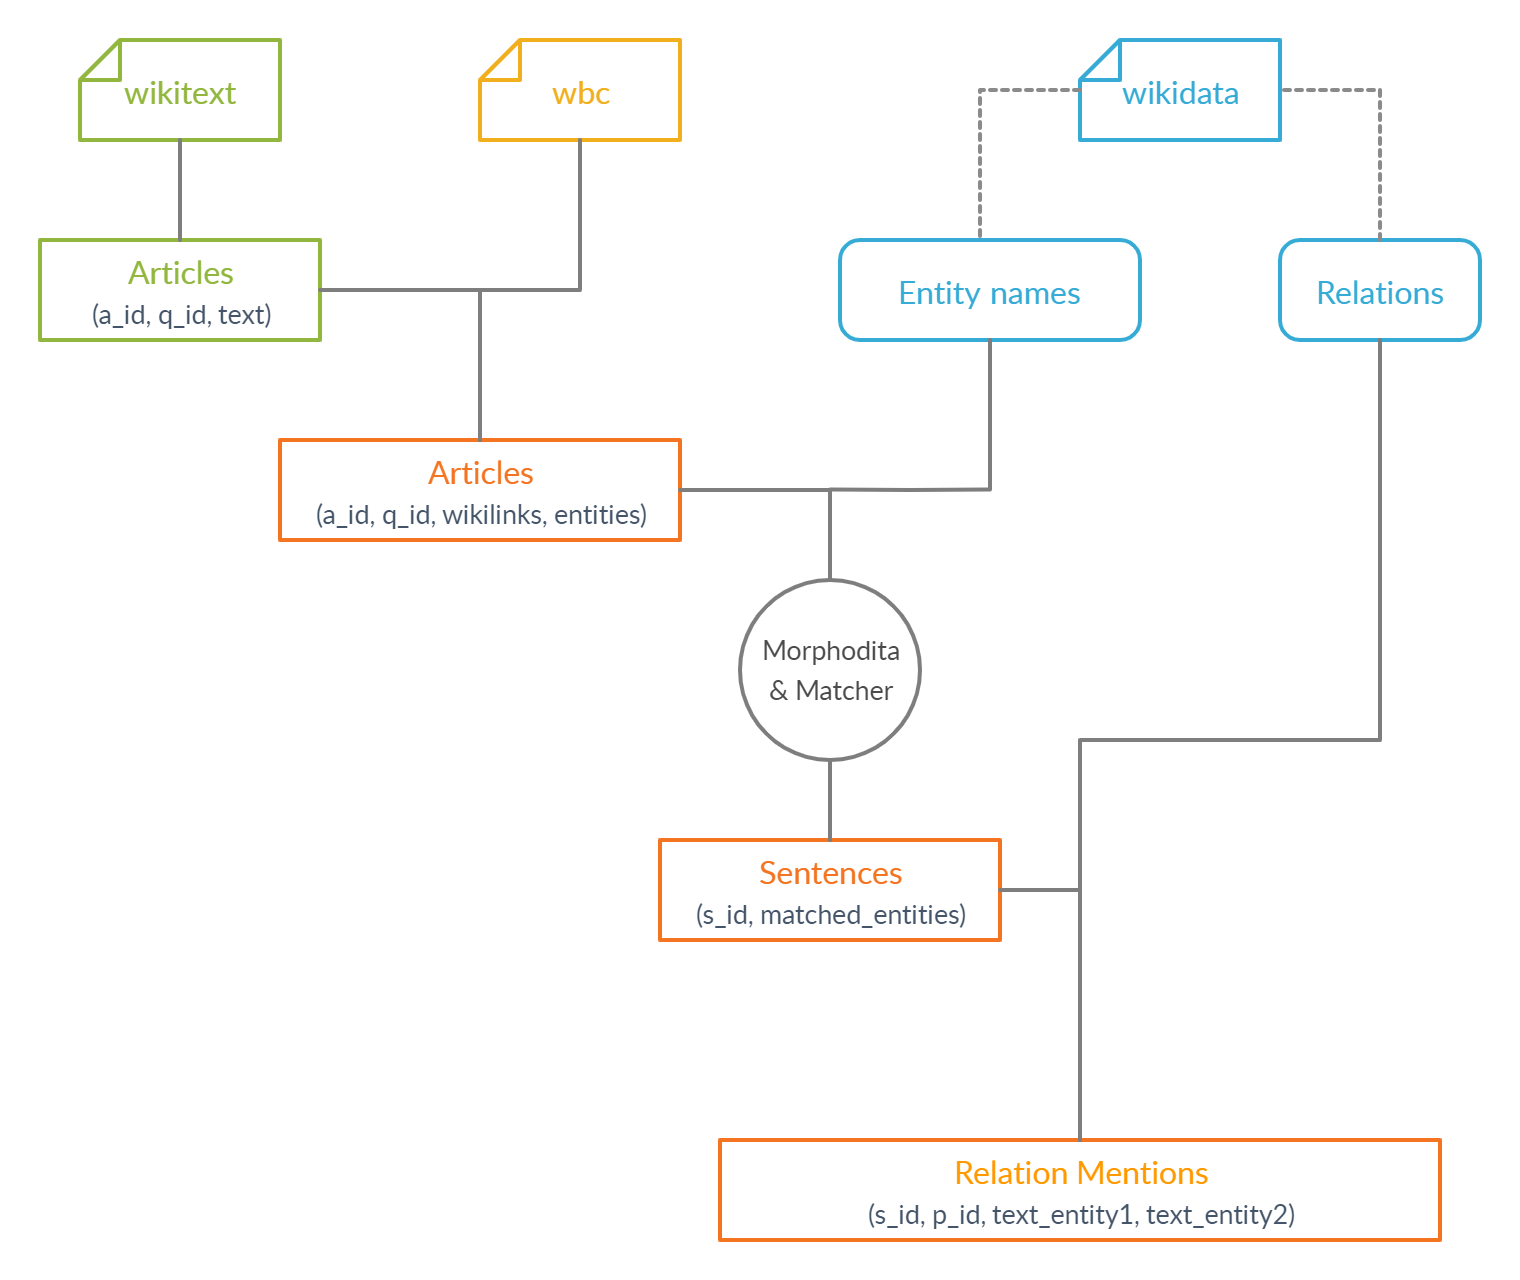
\includegraphics[width=140mm, height=117mm]{./img/Corpus_diagram}
\caption{Zjednodušený diagram výroby korpusu}
\label{obr03:Nhust}
\end{figure}


\section{Title of the second subchapter of the second chapter}


\chapter*{Conclusion}
\addcontentsline{toc}{chapter}{Conclusion}
In this thesis, we proposed a methodology for generating relationship extraction datasets using Wikipedia and Wikidata. We analysed different pitfalls that we faced when we implemented the generator and generated CERED (Czech Relationship Extraction Dataset). 

We designed a neural network architecture for the relationship extraction task. In the network, we employ BERT, which increases the quality of the network. We demonstrated that the proposed architecture preforms not much worse than the state-of-the-art on multiple English relationship extraction datasets. We reported the performance of the network on CERED.


\section{Future work}

\subsection{Other Languages}

This thesis focused on relationship extraction in the Czech  Language. We believe that our work could be extended into different languages. In the CERED generation process, there are three language-dependent steps:
\begin{itemize}
\item Wikidata preprocessing - we only worked with items, that had at least one Czech name. The filtering can be easily changed to arbitrary language. For languages with small Wikipedia, it might be reasonable to consider relaxing the condition.
\item Wikitext parsing - names of templates are in the language of the Wikipedia. We can remove the content of all templates. It will negatively impact the size of the dataset, but it too drastically.
\item Entity matching - this step is heavily dependant on the language. We believe that for some languages it might be satisfactory to change the language in MorphoDiTa (for example MorphoDiTa supports the Slovak language). We might consider exchanging MorphoDiTa with a more mainstream tool (for example, spaCy) that supports more languages.

\end{itemize}

If we implemented the changes proposed above and automatised the whole process, we might be able to create a dataset (and a model) for each language, that the multilingual BERT supports (coincidentally BERT was trained on the 100 biggest Wikipedias).

\subsection{Wikidata ontology}
In section \nameref{sec:otherconsideredvariations}, we mentioned that additional information for training could be obtained from wikidata. Such information is often available in other relationship extraction dataset. In the future, we would like to use Wikidata for extracting such information and add it to CERED.




%%% Bibliography
%%% Bibliography (literature used as a source)
%%%
%%% We employ bibTeX to construct the bibliography. It processes
%%% citations in the text (e.g., the \cite{...} macro) and looks up
%%% relevant entries in the bibliography.bib file.
%%%
%%% The \bibliographystyle command selects, which style will be used
%%% for references from the text. The argument in curly brackets is
%%% the name of the corresponding style file (*.bst). Both styles
%%% mentioned in this template are included in LaTeX distributions.

\bibliographystyle{plainnat}    %% Author (year)
% \bibliographystyle{unsrt}     %% [number]

\renewcommand{\bibname}{Bibliography}

%%% Generate the bibliography. Beware that if you cited no works,
%%% the empty list will be omitted completely.

\bibliography{bibliography}

%%% If case you prefer to write the bibliography manually (without bibTeX),
%%% you can use the following. Please follow the ISO 690 standard and
%%% citation conventions of your field of research.

% \begin{thebibliography}{99}
%
% \bibitem{lamport94}
%   {\sc Lamport,} Leslie.
%   \emph{\LaTeX: A Document Preparation System}.
%   2nd edition.
%   Massachusetts: Addison Wesley, 1994.
%   ISBN 0-201-52983-1.
%
% \end{thebibliography}


%%% Figures used in the thesis (consider if this is needed)
%\listoffigures

%%% Tables used in the thesis (consider if this is needed)
%%% In mathematical theses, it could be better to move the list of tables to the beginning of the thesis.
%\listoftables

%%% Abbreviations used in the thesis, if any, including their explanation
%%% In mathematical theses, it could be better to move the list of abbreviations to the beginning of the thesis.
%\chapwithtoc{List of Abbreviations}

%%% Attachments to the master thesis, if any. Each attachment must be
%%% referred to at least once from the text of the thesis. Attachments
%%% are numbered.
%%%
%%% The printed version should preferably contain attachments, which can be
%%% read (additional tables and charts, supplementary text, examples of
%%% program output, etc.). The electronic version is more suited for attachments
%%% which will likely be used in an electronic form rather than read (program
%%% source code, data files, interactive charts, etc.). Electronic attachments
%%% should be uploaded to SIS and optionally also included in the thesis on a~CD/DVD.
%%% Allowed file formats are specified in provision of the rector no. 72/2017.
\appendix
\chapter{Attachments}

\section{First Attachment}

\openright
\end{document}
